\chapter{The Influence Mining Framework}
\label{chp:inf-framework}
Influence Maximization has been proven as holy grail specially for viral marketing applications, thus attracting more than a handful of researchers who have proposed a wide variety of techniques, which are all applicable based on the nature of network they are applied to. However, Thorough analysis of the influence mining problem suggests that due to inherent constraints and network dynamics, it is not possible to suggest an ideal method or technique which is both realistic as well as optimal on all complex networks. This problem is accurately illustrated in a recent paper \cite{arora2017}. The authors show that if Quality, Efficiency and Memory consumption are three criteria to decide which algorithm best solves the influence maximization problem, then all the available state-of-art methods either fulfill one or two criteria. An algorithm which satisfies all three does not yet exist (see Figure \ref{fig:state-of-art-im-methods}\cite{arora2017}). One of the major reasons -- as discussed in Chapter \ref{chp:inf-max} -- behind this bottleneck is the structural variety in complex networks.

\begin{figure}[h]
	\centering
	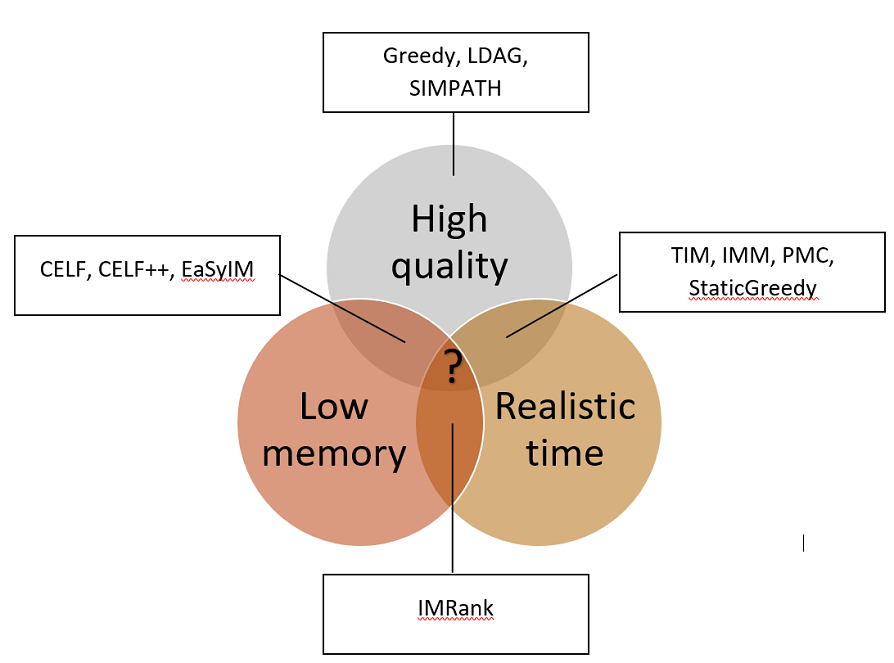
\includegraphics[width=0.7\textwidth]{state-of-art-im-methods}
	\caption[Deficiency in current state-of-art methods]{Several state-of-art methods and their primary objectives. The question mark denotes that no method exists to target all three criteria.}
	\label{fig:state-of-art-im-methods}
\end{figure}


	\section{Limitations of State-of-the-Art Methods}
	\label{sec:inf-framework-statofart-limitation}
	
		\subsection{Customary stoppage criteria}
		\label{subsec:inf-framework-stop-criteria}
		In lieu of an ideal influence maximization solutions, the applications are forced to adopt one algorithm. It is realistically challenging to apply one technique not only on a specific type of network, but also for varying use cases.
		
		First example in this regard is seasonal marketing campaigns. A business launching a new seasonal product will have a short time window to market and propagate their product before the competition launches more options, or the trend wears out. In this case, the business may allocate high budget, and may also overlook the magnitude of gain. However, the \textit{time} is real constraint and after the given window is passed, more efforts to maximize their influence will have significantly less gain against the effort put.
		
		In a different scenario, consider an automobile business introducing their first autonomous car after years of heavy investment on research and development. Once their prototype passes the quality testing phase, they produce a limited number of units to send to the independent press and reviewers before launch. In this particular case, the influence mining problem will have a classic criteria, i.e. \textit{budget}. The time it takes to find the influential nodes in their network of users will be of less relevance. The primary focus will be to discover $k$ people which will maximize their product's influence as much as possible.
		
		Another example can be from national health systems. A country's immunization program is committed to mitigating an emerging contagious disease. Their focus will likely be to immunize densely populated areas, which makes \textit{spread} the key indicator. In this case, it is possible to extend the budget as well as time to reach the goal, but the minimum spread will be they main constraint.
		
		The problem being highlighted in all of these examples is that the influence mining methods operate solely on one stoppage criteria, i.e. \textit{Budget}, while in reality, this is applicable only to a subset of the applications.
		
		\subsection{Influence quantifier}
		\label{subsec:inf-framework-influence-quantifier}
		The other major limitation we observe is that there exist two different domains of applications which quantify the influence differently. The first one is the most common and is interchangeably termed as \textit{spread} and \textit{diffusion}. The spread measures how an action or event propagated itself from the seed nodes into the network. This quantifier is most widely used in applications involving social networks. Second one is \textit{resilience}, which has been thoroughly discussed in previous chapter. This quantifier simulates the decomposition of a network, i.e. how a network is impacted when a set of influential nodes are removed from it. This quantifier is seen mostly in conventional graph applications like Computer and transport networks.
		
		The separation of both of these quantifiers have not only made the experiments that these quantifiers were used in secluded from each other, but have also left a gap in bench marking novel methods. These quantifiers can be unified by asking a simple question: are influential nodes resilient (and vice versa)?


	\section{Proposed Framework}
	\label{sec:inf-framework-proposed-framework}
	We propose a solution to attack both of the aforementioned problems by devising a flexible framework, which can be tuned on multiple stoppage criteria, thus providing a realistic approach for influence mining. Secondly, by unifying the quantifier functions of spread and resilience tests, the framework also offers more accurate bench marking tool to fit the application specific needs.
	
	\textbf{Resilience problem reformation}:
	%\label{sec:inf-framework-resilience-reformation}
	As a pre-requisite step, we redefine the problem of resilience in similar fashion as the Influence problem. Given an undirected graph $G=(V,E)$, the objective is to compute resilience $R(G)$ using a network dismantling method $M$, such that it minimizes the size of largest remaining sub-graph after removing exactly $k$ nodes. This altered definition deviates from the original problem in at least two ways:
		
	\begin{enumerate}
		\item In the resilience problem, the objective is to identify the most optimal \textit{function} to dismantle a network. In our definition, the objective is to identify a set of most optimal $k$ nodes.
		
		\item The network decomposition continues in the original problem for all connected components. The redefined definition only concerns with the largest connected component.
	\end{enumerate}
	
	This simple reformation enables us to directly map any resilience application with influence mining.

	\begin{algorithm}[h]
		\caption{Proposed Influence Mining framework with flexible stoppage criteria}
		\label{alg:influence-mining-framework}
		\SetAlgoLined
		\KwInput{A connected network $G$ as a set of $V$ vertices and $E$ edges; a seed selection algorithm $M$; a criteria function $\rho$; threshold parameter $\theta$ for criteria function; and an influence quantifier function $\sigma$)}
		\KwOutput{$S;\sigma(S)$ (the set of influential nodes; approximate influence)}
		$S \gets \emptyset$
		\newline
		\While{$\rho(S)\leq \theta$}{ (until the value calculated by criteria function is below threshold)
			$S \gets S\cup M(G,V-S)$ (add nodes to the influential set returned by seed selection algorithm)
		}
		\Return{$S;\sigma(S)$} (return the set of influential nodes and their total influence)
	\end{algorithm}

	The proposed algorithm (see \ref{alg:influence-mining-framework}) uses a graph $G=(V,E)$ as input, similar to any influence algorithm. The second parameter $M$ represent the method to calculate the importance, or vitality of a node. A variety of such methods are briefly discussed in \ref{sec:related-seed-selection}. The third parameter, $\rho$ is a function which defines a criteria to halt the influence mining process and return the set of influential nodes $S$ found. $\theta$ is the threshold or cut-off value for $\rho$ function where the process will halt. Finally, $\sigma$ is the function to quantify the magnitude of influence. For an insight, we enlist a few types of criteria parameters:
		
	\begin{enumerate}
		\item Budget $k$. Number of nodes in the seed set reaches $k$, regardless of the running time and their spread. This is the de facto criteria for all of the influence maximization solutions due to which the selection of right budget is a debatable topic. Pareto principle \cite{pareto1971} suggests that the budget should be 20\%, while \cite{kempe2003} argue that this number is much smaller. Leskovec et al. \cite{leskovec2007b} showed that the growth in gain with respect to budget is logarithmic.
		
		\item Allowed time $t$ for computation. If the running time approaches $t$, then the convergence is assumed.
		
		\item Minimum spread $S_{min}$. If the set of influential nodes identified have expected spread of $\sigma(S)\ge S_{min}$
		
		\item At least $c$ percent network coverage achieved. On larger networks, it is often not possible to make an influence attempt on every node, therefore the convergence criteria is set to the percentage of network reached during the diffusion process.	
	\end{enumerate}

	This framework provides a platform for influence mining applicaitons by adding two novel ingredients, the stoppage criteria and custom quantifier. Any implementation built on top of this framwork will provide flexibility to incorporate more real-life use cases than the old architecture permitted. In the next section we now put this framework to test on multiple criteria to validate whether this framework actually meets these expectations.


	\section{Validation of Influence Mining (IMine) Framework}
	\label{sec:inf-framework-validation}
	This series of experiments comprehensively evaluates the proposed IMine Framework from various aspects. While IMine is liberal in accepting the stoppage function and its respective threshold value, we will evaluate it using the aforementioned Budget, Allowed Time and Minimum Spread parameter functions. Moreover, both resilience and diffusion quantifiers are used to benchmark the accuracy of underlying models.
	
		\subsection{Data set}
		The data set consists of 28 undirected complex networks with varying properties; the rationale behind using such a large number is to mitigate any bias. We include all the networks used in previous findings in this thesis. The networks are listed below, while their statistics can be seen in Tables \ref{tab:inf-framework-network-stats-a} and \ref{tab:inf-framework-network-stats-b}:
		
		\begin{itemize}
			\item ArXiv collaboration (arxiv)\cite{leskovec2007c}: a collaboration graph crawled from arXiv.org, High Energy Physics and Physics section.
			
			\item Author NetScience (author)\cite{newman2006b}: a co-authorship network of scientists working on network theory and experiments, as compiled by M. Newman in 2006.
			
			\item Automata GraphDraw (automata)\cite{eades1996}: a finite automaton used in a natural language processing system, provided by Emmanuel Roche in graph drawing contest in 1996.
			
			\item AS-Caida (caida)\cite{leskovec2007c,ascaida}: network of autonomous systems of the Internet connected with each other from the CAIDA project, collected in 2007. Nodes are Autonomous Systems (AS), and edges denote communication.
			
			\item City Economic Networks (city2010 - city2019): see \ref{sec:resilience-city-networks}.
			
			\item Epinions.com (epinions)\cite{richardson2003}: an online who-trust-whom social network for consumers who give reviews to several goods.
			
			\item Facebook TV shows (fb\_tvshows)\cite{rossi2015}: network of Facebook TV show pages mutually liked by users collected using GraphViz, an interactive network data visualization and analytics platform.
			
			\item Football games (football)\cite{girvan2002}: American football games between Division IA colleges during regular season Fall 2000.
			
			\item Influence citations (influence\_citation): see \ref{sec:inf-max-machine-learning}.
			
			\item ITA-2000 (ita2000)\cite{rozenblat2008}: Air Transport network representing connections between airports through direct flights. The network used is a reduced subgraph of original network.
			
			\item Java Development Kit 6 Classes(jdk6)\cite{jdk}: Java class dependency network of JDK framework v1.6. Nodes represent classes and edges represent dependency between two classes.
			
			\item Johns Hopkins University Facbook Network (johnshopkins)\cite{ryan2015}: social friendship network of Facebook from pupils studying in Johns Hopkins university, extracted in the year 2012.
			
			\item Karate club (karate)\cite{zachary1977}: social network of members of a karate club at an American University. The network represents ties between members of the club based on their social interactions.
			
			\item Linux source code (linux)\cite{linux}: this is the network of Linux source code files in which each node is a file and edges represent interactions between these files.
			
			\item Moreno Student–student friendships (moreno)\cite{moody2001}: a network from a survey in which students were asked to list 5 best male/female friends. A node represents a student and an edge between two students shows that the left student chose the right student as a friend.
			
			\item Neural Network of Nematode (nematode)\cite{white1986}: neural network of the nematode from original experimental data by White et al.
			
			\item Petster-hamster (hamster)\cite{hamster}: friendship network of hamster adopters from popular pet website, Petster.com.
	
			\item Political Blogs (political)\cite{adamic2005}: a network of hyperlinks between weblogs on US politics, which comes from from blog directories. Blogs were labeled based on incoming/outgoing edges and posts around the 2004 presidential election in USA.
			
			\item Spam on Web Challenge (spam)\cite{castillo2008}: network submitted by Castillo et. al. in Web spam challenge 2008.
			
			\item Tech Routers(routers)\cite{spring2002}: a collection of tech router links, collected to measure the topology of Internet service providers with Rocketfuel, a technology company based in USA.
	
			\item US Airport (usairport)\cite{opsahl-usairport}: network of flights between US airports in 2010. An edge represents a connection from one airport to another, original network is weighted but in the experiments, the weights are normalized.
			
			\item Word Net (wordnet)\cite{fellbaum2012}: a lexical network of English words in which each node represents a word and edges are relationships like synonym and antonyms.
			
			\item World Trade (world\_trade)\cite{smith1992}: network of flow of global commodity trade. The data was used by Smith et. al. for quantitative analysis of the global economic system, particularly to identify the roles that countries play in the division of labour.
			
			\item Yeast Protein (protein)\cite{jeong2001}: Protein-protein interaction network of yeast. % This network is widely used in studies like \cite{barabasi2002,boccaletti2006}.
		\end{itemize}
		
		\begin{longtable}[c]{|l|l|l|l|l|l|l|l|}
			\hline
			\textbf{graph}      & \textbf{edges} & \textbf{nodes} & \textbf{ratio} & \textbf{avg\_deg} & \textbf{apl} & \textbf{high\_deg} & \textbf{diameter} \\ \hline
			\endfirsthead
			%
			\endhead
			%
			arxiv               & 41602          & 6794           & 0.163          & 12.25             & 5.780        & 341                & 16                \\ \hline
			author              & 914            & 379            & 0.415          & 4.82              & 6.042        & 34                 & 17                \\ \hline
			automata            & 2770           & 1096           & 0.396          & 5.05              & 1.995        & 1096               & 2                 \\ \hline
			caida               & 53381          & 26475          & 0.496          & 4.03              & 3.876        & 2628               & 17                \\ \hline
			city2010            & 39904          & 1209           & 0.030          & 66.01             & 2.287        & 1045               & 5                 \\ \hline
			city2013            & 49926          & 1358           & 0.027          & 73.53             & 2.268        & 1154               & 4                 \\ \hline
			city2016            & 62523          & 1405           & 0.022          & 89.00             & 2.264        & 1188               & 5                 \\ \hline
			city2019            & 68668          & 1422           & 0.021          & 96.58             & 2.244        & 1258               & 5                 \\ \hline
			epinions            & 508836         & 75877          & 0.149          & 13.41             & 4.308        & 3079               & 15                \\ \hline
			fb\_tvshows         & 17262          & 3892           & 0.225          & 8.87              & 6.276        & 126                & 20                \\ \hline
			football            & 616            & 115            & 0.187          & 10.71             & 2.508        & 13                 & 4                 \\ \hline
			hamster             & 12476          & 1788           & 0.143          & 13.96             & 3.453        & 272                & 14                \\ \hline
			influence\_citation & 1993           & 1254           & 0.629          & 3.18              & 3.806        & 172                & 6                 \\ \hline
			ita2000             & 67195          & 3304           & 0.049          & 40.67             & 4.037        & 1826               & 13                \\ \hline
			jdk6                & 150985         & 6434           & 0.043          & 46.93             & 2.120        & 32530              & 7                 \\ \hline
			johnshopkins        & 186572         & 5157           & 0.028          & 72.36             & 2.710        & 886                & 8                 \\ \hline
			karate              & 78             & 34             & 0.436          & 4.59              & 2.408        & 17                 & 5                 \\ \hline
			linux               & 230201         & 30817          & 0.134          & 14.94             & 3.254        & 9775               & 12                \\ \hline
			moreno              & 12969          & 2539           & 0.196          & 10.22             & 4.559        & 36                 & 10                \\ \hline
			nematode            & 2359           & 297            & 0.126          & 15.89             & 2.455        & 139                & 5                 \\ \hline
			political           & 19089          & 1222           & 0.064          & 31.24             & 2.738        & 468                & 8                 \\ \hline
			protein             & 3941           & 1458           & 0.370          & 5.41              & 6.812        & 112                & 19                \\ \hline
			routers             & 6632           & 2113           & 0.319          & 6.28              & 4.607        & 109                & 12                \\ \hline
			spam                & 37375          & 4767           & 0.128          & 15.68             & 3.794        & 477                & 12                \\ \hline
			usairport           & 28235          & 1572           & 0.056          & 35.92             & 3.115        & 596                & 8                 \\ \hline
			wordnet             & 656230         & 145145         & 0.221          & 9.04              & 5.532        & 1008               & 16                \\ \hline
			world\_trade        & 1000           & 80             & 0.080          & 25.00             & 1.724        & 95                 & 3                 \\ \hline
			\caption{Network statistics of all networks included in the experiment. Edges represents number of undirected edges; nodes represents the size; ratio is ratio between nodes and edges; avg\_deg is average degree of nodes; apl is average path length; high\_deg is the highest degree; avg\_dist is average distance; triads is the number of triads in the network and power\_law is the coer}
			\label{tab:inf-framework-network-stats-a}\\
		\end{longtable}
		
		\begin{longtable}[c]{|l|l|l|l|l|l|}
			\hline
			\textbf{graph}      & \textbf{transitivity} & \textbf{assortativity} & \textbf{avg\_dist} & \textbf{triads} & \textbf{power\_law} \\ \hline
			\endfirsthead
			%
			\endhead
			%
			arxiv               & 0.19831               & 0.376                  & 5.780              & 45000           & 4.20                \\ \hline
			author              & 0.43058               & -0.082                 & 6.042              & 2763            & 3.36                \\ \hline
			automata            & 0.00556               & -0.746                 & 1.995              & 6987            & 3.46                \\ \hline
			caida               & 0.00732               & -0.195                 & 3.876              & 109095          & 2.09                \\ \hline
			city2010            & 0.34313               & -0.241                 & 2.287              & 2021343         & 2.10                \\ \hline
			city2013            & 0.34883               & -0.251                 & 2.268              & 2931834         & 6.12                \\ \hline
			city2016            & 0.38030               & -0.222                 & 2.264              & 4223793         & 2.21                \\ \hline
			city2019            & 0.39310               & -0.206                 & 2.244              & 4932006         & 5.93                \\ \hline
			epinions            & 0.06568               & -0.011                 & 4.308              & 4873443         & 1.70                \\ \hline
			fb\_tvshows         & 0.59064               & 0.561                  & 6.276              & 261270          & 2.75                \\ \hline
			football            & 0.40724               & 0.142                  & 2.508              & 2430            & 21.19               \\ \hline
			hamster             & 0.09037               & -0.089                 & 3.453              & 50223           & 4.32                \\ \hline
			influence\_citation & 0.05710               & -0.407                 & 3.806              & 3537            & 2.35                \\ \hline
			ita2000             & 0.24894               & 0.007                  & 4.037              & 302496          & 1.69                \\ \hline
			jdk6                & 0.01110               & -0.223                 & 2.120              & 584526          & 2.01                \\ \hline
			johnshopkins        & 0.19316               & 0.080                  & 2.710              & 4943352         & 5.57                \\ \hline
			karate              & 0.25568               & -0.476                 & 2.408              & 135             & 2.13                \\ \hline
			linux               & 0.00282               & -0.175                 & 3.254              & 512586          & 1.96                \\ \hline
			moreno              & 0.14189               & 0.288                  & 4.559              & 14082           & 8.42                \\ \hline
			nematode            & 0.18071               & -0.150                 & 2.455              & 9723            & 3.29                \\ \hline
			political           & 0.22596               & -0.196                 & 2.738              & 303129          & 3.89                \\ \hline
			protein             & 0.05178               & -0.207                 & 6.812              & 618             & 3.24                \\ \hline
			routers             & 0.22826               & 0.019                  & 4.607              & 31212           & 2.74                \\ \hline
			spam                & 0.14519               & 0.000                  & 3.794              & 387051          & 2.42                \\ \hline
			usairport           & 0.38414               & -0.122                 & 3.115              & 735516          & 1.86                \\ \hline
			wordnet             & 0.09575               & -0.063                 & 5.532              & 3433944         & 2.47                \\ \hline
			world\_trade        & 0.45957               & -0.294                 & 1.724              & 13299           & 2.56                \\ \hline
			\caption{Network statistics of all networks included in the experiment. avg\_dist is average distance; triads is the number of triads in the network and power\_law is the coefficient $\alpha$ of power law}
			\label{tab:inf-framework-network-stats-b}\\
		\end{longtable}
	
		\subsection{Analysis of Data set}
		The networks used are a wide range of complex network types of varying sizes and structural attributes. We used five small networks of sizes under 1000 nodes, eighteen medium-sized networks under 10000 nodes, and five large networks with over 10000 nodes. Besides the size and volumes of the networks, we examine a few key metrics which can be a good criteria to establish that the data set indeed offers variations:
		
		\begin{enumerate}
			\item Node-edge ratio is a good indicator of how densely the network is connected. Lower value indicates that there are few nodes, but are tightly connected with each other. Similarly, value close to 1 indicates that the network is loosely connected with nodes only linked with few neighbours. The boxplot \ref{fig:inf-framework-networks-ratio} illustrates that this value lingers between 0.2 and 0.3\footnote{the distance between median and mean values in the plot are due to unusually high ratio in influence\_citation}. Average degree is another metric which tells the extent to which the nodes are interconnected in a network. Boxplot \ref{fig:inf-framework-networks-avg-degree} illustrates the measure of central tendency for average degree.
			
			\item It has been discussed in initial chapters that APL is among the key metrics to understand the reach from node to node in a network. Figure \ref{fig:inf-framework-networks-apl} shows that apart from protein network, all networks follow 6-degree separation rule, i.e. they are small-world networks.
			
			\item Diameter, a metric which is closely related to the coreness of a network is a good way to understand whether the graph is centralized to a single core or decentralized. The data set has a broad range of diameters from 2 to 20, which guarantees that not all the networks in our data set are structurally identical. Bar plot \ref{fig:inf-framework-networks-diameter} details about the diameter distribution in a glance. Again, the networks cover a broad range from 2 to 20 in diameter measure.
			
			\item On transitivity, only fb\_tvshows has an unusually high value of transitivity (0.59), the networks are majorly ranging between 0.15 and 0.35 (see Figure \ref{fig:inf-framework-networks-transitivity}). The higher value means tighter clique-like structure.
			
			\item Assortativity tells whether nodes are following preferential attachment. A negative value tells that high-degree nodes are connecting with low-degree nodes while a positive value tells high-degree nodes prefer to connect with other high-degree nodes. A dynamic graph, by definition is the one which changes over time, and assortativity tells us exactly "how" a graph will look like in the future by looking at current assortativity coefficients of nodes. Hence this is a unique metric which can be used to understand dynamic properties of a graph, for example against a targeted attack a highly assortative network will be infected completely differently than a low assortative network. We note that the data set covers a wide spectrum of networks with a few highly assortative, few highly disassortative, and several low assortative/disassortative networks; this is shown in histogram \ref{fig:inf-framework-networks-assortativity}.
			
			\item Looking at the power-law, the minimum, mean, maximum and outlier values are 1.69, 3.23, 8.42, 21.19 respectively. Thus indicating that most of the networks follow power-law distribution. All the power law degree-probability distribution plots can be found in Appendix \ref{sec:appendix-C-inf-framework}.
		\end{enumerate}
		
		\subsection{Experiment settings}
		The experiments aim to evaluate two novelties which the IMine Framework proposes. First is to test whether the claim that influence mining methods perform differently on changing stoppage criteria holds true or not. Second objective is to check if the diffusion and resilience tests can be used simultaneously for influence benchmarking/quantification.
		
		The IMine Framework is not specific to a closed set of criteria, however we will evaluate the framework for \textit{Budget} and \textit{Influence} in our experiments.
		
			\subsubsection{Hypothesis 1}
			The performance of an algorithm varies on the same set of networks for different stoppage criteria. The $H_{1_0}$ for this hypothesis is: \textit{Accuracy of an algorithm is independent of stoppage criteria}. Whereas the alternate hypothesis $H_{2_A}$ is: \textit{Accuracy of an algorithm is not independent of stoppage criteria}.

			We try each algorithm on the aforementioned stoppage criteria and measure the number of instances that each algorithm ranked on top on Budget, then count the number of instances where the same algorithm was not ranked on top for Influence criteria. This is repeated for each algorithm under observation. If the difference in the ranks on different budgets is statistically significant, then we reject the $H_{1_0}$.
			
			\subsubsection{Hypothesis 2}
			If the performance of an algorithm is high on diffusion test, then its performance will also hold on resilience test. The $H_{2_0}$ for this hypothesis is: \textit{There is no relationship between diffusion test and resilience test}. Whereas the alternate hypothesis $H_{2_A}$ is: \textit{Performance of an algorithm on diffusion test is similar to the performance on resilience test}.
			We measure the diffusion under IC and LT models as well as resilience when conducting experiments for the first objective. The number of instances where a method stood on top in the resilience test and diffusion test simultaneously is measured against the number of instances where it did not; $H_{2_0}$ is rejected if the similarity is statistically significant between both the counts.
			
			\subsubsection{Influence methods}
			As mentioned earlier, a mix of both classic and state-of-art methods will be used to mitigate the bias risk. Algorithms chosen for this experiment are:
			
			\begin{enumerate}
				\item Adaptive sampling variation of Degree, Betweenness, Closeness and Eigenvector centrality methods.
				
				\item Pagerank
				
				\item K-core decomposition
				
				\item Collective influence
				
				\item Greedy CELF\footnote{we opted against the improved version, i.e. CELF++ due to its inconsistency in IC versus LT models\cite{arora2017}.}
			\end{enumerate}
			
			\subsubsection{Ranges of stoppage criteria}
			Instead of working on fixed value of criteria, we revise the experiments for different values in order to get a fair aggregate of observations.
			
			\begin{itemize}
				\item Budget: for smaller graphs, the value set of budget is \{1\%, 2\%, 3\%, 4\%, 5\%\} for networks under 10,000 nodes and \{1.25\%\} for larger networks.
				
				\item Influence Spread: the value set for influence relative to the size of the network is \{0.5\%, 1\%, 3.3\%, 6.7\%, and 10\%\}, i.e. spread up to one tenth of the network. For networks of sizes over 10,000 nodes, the value set is \{0.5\%, 1\%, and 2.5\%\}.
			\end{itemize}
			
			\subsubsection{Identifying the best algorithm}
			The notion of best algorithm is used when referring an influence method, which identifies a set of nodes with maximum gain with respect to criteria. If the criteria is to stop as fast as possible, then the best algorithm will be the one which ends the influence process faster than the others. Similarly, if the criteria is to gain maximum influence then the algorithm which identifies nodes with maximum influence qualifies as the best method. Criterion is the key to define what qualifies as value gain:
			
			\begin{itemize}
				\item Budget: when the input criteria is Budget, then the best algorithm will be the one which mines the set of most influential nodes of size $k$, irrespective of cost in terms of spread $\sigma$. Here, we quantify influence for various sets of nodes and pick a set which maximizes the influence spread. For example, the input to the IMine framework could be: $G:(1000,1500); M=PageRank; \rho=budget; \theta =0.5\%; \sigma=influence$. The output will be a set of nodes like $S=\{5,13,100,410,875\}$ and their influence measure $\sigma(S)=60$. In this case, the process continues to run until convergence, i.e. the size $|S|$ reaches the threshold $\theta$.
				
				\item Influence: for this criteria, an algorithm is labeled as best if it identifies a set of nodes which achieves a minimum Influence spread of the threshold value supplied, irrespective of time taken and size of the node set, meaning $k$ is not fixed.
				
				For example, the input to the IMine framework could be: $G:(1000,1500); M=PageRank; \rho=influence; \theta=100; \sigma=influence$. The output will be a set of nodes like $S=\{5,13,100,410,875,890,988\}$ and their influence measure $\sigma(S)=110$. In this case, the process continues to run until convergence, i.e. the influence $\sigma(S)$ exceeds the threshold $\theta$. Note that the size $|S|$ was not restricted in this case.
			\end{itemize}
			
			\subsubsection{Identifying worst algorithm}
			Synonymous to the prior description, worst algorithm refers to the algorithm which identifies the set of nodes with maximum cost associated than the other methods used for comparison. It is important to note that the evaluation of cost is two-factored in some cases. For example, if more than one algorithms prove to be on the same level in terms of influence, then the additional deciding factor of time is added to break the tie. In case of Budget, if two or more algorithms result in same set of nodes, or the influence measure is same, then the algorithm which also took more time to execute is labeled as worst algorithm. On the other hand, to break the tie for Influence criteria, the algorithm which took more time to execute is selected.
	
			\subsubsection{Identifying most efficient/inefficient algorithm}
			While conventionally, the efficiency is measured using the time complexity of algorithms, in a comprehensive experiment as such, there are numerous factors involved when calculating the time complexity of an algorithm on a particular graph. Therefore a simplified formula of efficiency is devised which calculates cost per unit gain in influence, i.e. $\eta(M)=\frac{\sigma(S)}{t}$ where $\sigma(S)$ denotes the influence measure of the algorithm and $t$ is the elapsed time in seconds. The higher this ratio, the more efficient an algorithm and vice versa.
			
		\subsection{Results}
		The experiment results encompass the two hypothesis ($H_{1_0}$ and $H_{2_0}$), as well as individual performances of each influence method in terms of both Accuracy and Efficiency - best and worst cases\footnote{The figures shown in this section are summaries, please refer to Appendix subsection \ref{subsec:appendix-imine-evaluation} for detailed results}.
	
			\subsubsection{Performance evaluation - accuracy}
			Figures \ref{fig:inf-summary-budget} and \ref{fig:inf-summary-influence} illustrate the distribution of methods with their respective \textit{win} percentages, i.e. how many times they outperformed other methods in a given stoppage criteria. These numbers are aggregate of results for all test methods. Figure \ref{fig:inf-summary-value-distribution} plots the efficiency of each method\footnote{Only the methods which outperformed others in at least 1 instance are shown}.
			
			When analyzing the accuracy of each method for budget criteria, we observe that Pagerank surpassed other methods by a monumental margin, i.e. in 51\% trials. Adaptive Degree 11\% and CELF-greedy 10\% ranked second and third with slight margin. For the influence criteria, the results hang more in balance; Adaptive Eigenvector centrality takes the lead with 21\% followed by CELF-greedy with 20\%, then finally Adaptive Degree with 13\%. Note that Pagerank resulted third last in this instance. It is also transparent that not only the best performing methods change their ranking where the criteria is changed, the methods performing worst also changed their ranks likewise. For the budget criteria, Adaptive Closeness performed worst with 2\%; Adaptive Eigenvector second to worst with 5\%; Adaptive Betweenness third worst with 6\%. For influence criteria, Collective influence finished last with 6\%; Pagerank second worst with 8\%; Coreness being third worst with 9\%.
			
			The argument behind IMine that there should be flexibility in the criteria, can be seen as becoming valid because Pagerank, which was the top performer for budget criteria performed poorly on Influence criteria. Similarly, the Eigenvector centrality, which was the second least accurate method for budget criteria came on top for influence criteria.
			
			\begin{figure}[H]
				\centering
				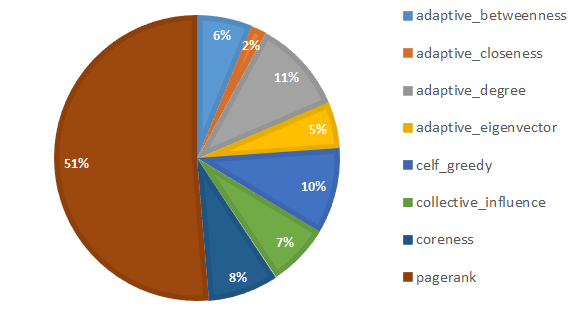
\includegraphics[width=1\textwidth]{inf-summary-budget}
				\caption[IMine performance summary on budget criteria]{Overall summary of percentages of instances in which each method outperformed the other methods in budget criteria. The method with most influence was selected as the best method.}
				\label{fig:inf-summary-budget}
			\end{figure}
			
			\begin{figure}[H]
				\centering
				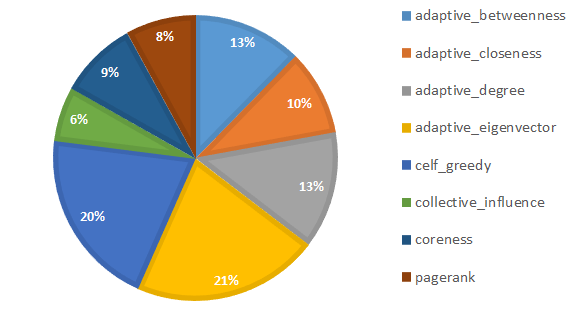
\includegraphics[width=1\textwidth]{inf-summary-influence}
				\caption[IMine performance summary on influence criteria]{Overall summary of percentages of instances in which each method outperformed the other methods in influence criteria. The method which took least time to reach was selected as the best method.}
				\label{fig:inf-summary-influence}
			\end{figure}
	
			\subsubsection{Performance evaluation - efficiency}
			Conventionally, the term efficiency refers to how quickly an action was performed. However, variation in size and type of networks in the data set makes it impractical to use time alone as a measure as the algorithm run time depends highly upon the structural properties; the efficiency is measured as the ratio between the influence and elapsed time, i.e. $\eta=\frac{\sigma}{t}$. The need for this metric can be understood through Figure \ref{fig:inf-summary-min-time}, which shows how frequent a method outperforms others in terms of minimum time. It can be observed that while Coreness has twice as many wins as compared to second best Pagerank algorithm, the percentages in \ref{fig:inf-summary-value-distribution} shows that it is only marginally ahead of Pagerank.
			
			Empirical analysis of results performed on efficiency can be viewed in figure \ref{fig:inf-summary-value-distribution}. The observations solidify the grounds which the IMine framework is built upon. When measuring the efficiency, no single method has significant lead over the others. The top performer, Coreness came out as most efficient in 33\% cases, followed by Pagerank with 27\% win percentage; and finally the Adaptive degree with 24\% winning ratio.
			%In contrast, the Pagerank algorithm had shown significant improvement over other methods in budget trials.
			
			\begin{figure}[H]
				\centering
				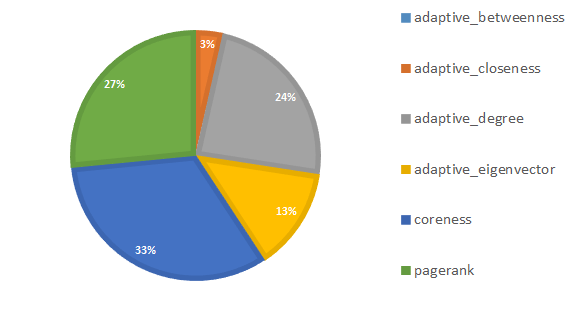
\includegraphics[width=1\textwidth]{inf-summary-max-value}
				\caption[IMine efficiency on influence criteria]{Overall summary of percentages of instances in which each method outperformed the other methods in terms of efficiency for influence criteria. The method with highest $\eta$ is selected as the most efficient method.}
				\label{fig:inf-summary-max-value}
			\end{figure}
	
			\begin{figure}[H]
				\centering
				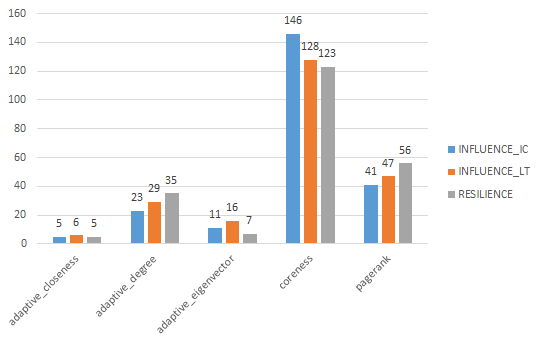
\includegraphics[width=1\textwidth]{inf-summary-min-time}
				\caption[IMine lowest time comparison]{Number of times each method executed in lowest elapsed time as compared to other methods, distributed by test method. The results from both budget and influence trials have been combined.}
				\label{fig:inf-summary-min-time}
			\end{figure}
			
		
			\subsubsection{Hypothesis 1}
			We established that for overall results, the performance of an influence method is not independent on the stoppage criteria, we now observe whether these results stand for all the three influence test methods or not. Figures \ref{fig:inf-summary-budget-distribution} and \ref{fig:inf-summary-influence-distribution} illustrate how the win instances for each method are distributed. 
	
			\begin{figure}[H]
				\centering
				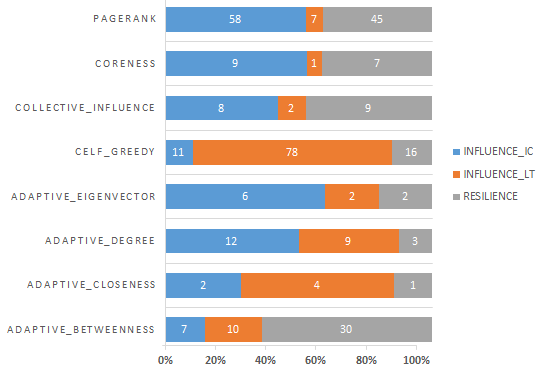
\includegraphics[width=1\textwidth]{inf-summary-budget-distribution}
				\caption[IMine performance on budget criteria on all test methods]{Percentage of number of instances each method outperformed the other methods in budget criteria, distributed by test method. The method with most influence was selected as the best method.}
				\label{fig:inf-summary-budget-distribution}
			\end{figure}
			
			\begin{figure}[H]
				\centering
				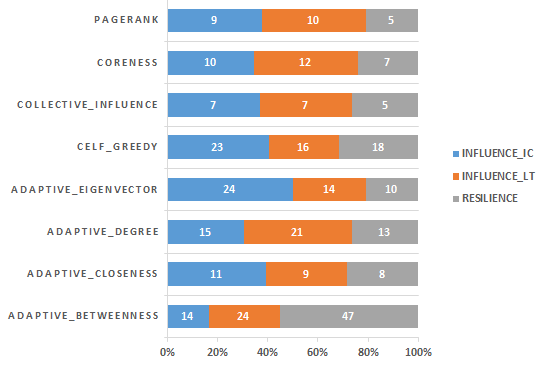
\includegraphics[width=1\textwidth]{inf-summary-influence-distribution}
				\caption[IMine performance on influence criteria on all test methods]{Percentage of number of instances each method outperformed the other methods in influence criteria, distributed by test method. The method with most influence was selected as the best method.}
				\label{fig:inf-summary-influence-distribution}
			\end{figure}		
	
			\begin{figure}[H]
				\centering
				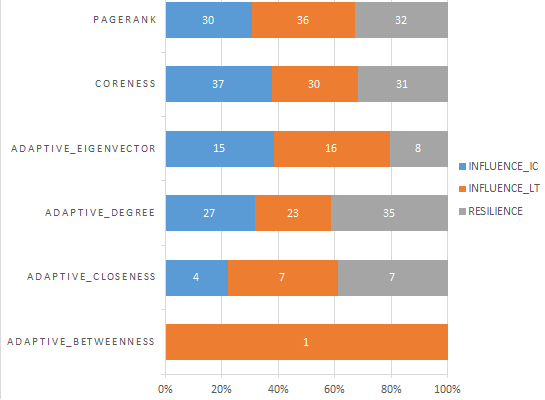
\includegraphics[width=1\textwidth]{inf-summary-value-distribution}
				\caption[IMine efficiency on all test methods]{Percentage of number of instances each method outperformed the other methods in efficiency criteria, distributed by test method. The method with highest efficiency was selected as the best method.}
				\label{fig:inf-summary-value-distribution}
			\end{figure}		
			
			Figures \ref{fig:inf-summary-budget-distribution} and \ref{fig:inf-summary-influence-distribution} are assessed in two stages, first we find the methods which performed well in each test method individually for budget criteria, then these findings are compared with the best performers for influence criteria. If the number of observations where a method that performed well for both criteria consistently is significant, the $H_{1_0}$ will be accepted.
			
			From figure \ref{fig:inf-summary-budget-distribution} we see that for Influence\_IC Pagerank stood as top performer with 58 observations (out of 113), followed by Adaptive Degree with 12 observations; for Influence\_LT, the CELF-greedy outperformed other methods by a wide margin with 78 observations, followed by Adaptive Betweenness with only 10 of such observations; finally, for the Resilience test the Pagerank algorithm again performed better than the rest with 45 observations, followed by Adaptive Betweenness with 30 observations.
			
			In figure \ref{fig:inf-summary-influence-distribution}, a different pattern is observed. For Influence\_IC test, Adaptive Eigenvector method came on top with 24 observations, followed by CELF-greedy only marginally behind with 23 observations. Neither Pagerank, nor Adaptive Degree performed as good as they did for budget criteria; for Influence\_LT, we see Adaptive Betweenness as the best performer with 24 observations, followed closely by Adaptive Degree with 21 wins. Again, the CELF-greedy algorithm which was highly dominant in former test did not perform anywhere close; for Resilience test, Adaptive Betweenness outperformed other methods with 47 observations, followed by CELF-greedy. Pagerank algorithm failed to enlist itself as a top performer.
			
			In a brief manner, for all the three test methods analyzed empirically for both the criteria, out of 12 cases (top 2 performers for all 3 methods on the 2 criteria), only once did we observe a consistent pattern where Adaptive Betweenness was 2nd best for budget and the best for influence criteria. We use Odds Ratio method to evaluate the significance:
			Let $O_{true}$ be the ratio of instances supporting $H_{1_0}$; $O_{false}$ be the ratio of instances against $H_{1_0}$; $N$ be the number of findings; $OR=\frac{O_{false}}{O_{true}}$. Hence, $OR=\frac{11/12}{1/12}=11$. In other words, the $H_{1_0}$ is 11 times unlikely to be true as compared to being false.
			
			We reject $H_{1_0}$ and accept $H_{1_A}$ since in no observation a method ranked similar when changing criteria\footnote{Significance testing is not required since the number of observations supporting the hypothesis is 0}. In the extended analysis, the $H_{1_0}$ is rejected as the Odds Ratio of the number of times an influence method performed consistently well to not performing consistently is 1 to 11.
			
			\subsubsection{Hypothesis 2}
			As stated before, the hypothesis is that there exists no relationship between diffusion and resilience test. We are confirming that both of these tests are indeed different and cannot be used interchangibly.
			
			Table \ref{tab:inf-framework-test-method-comparison} shows how frequently the trials supported $H_{2_1}$ in terms of percentages. The Resilience test is compared with both Influence tests individually as well as combined. The percentages show the ratio of trials in which one or more test methods matched. For example, for graph ArXiv on threshold 0.01, if the most influential method for Resilience test was CELF-greedy, and for Influence\_IC test was Pagerank, and for Influence\_LT was CELF-greedy, then "Resilience = Influence\_LT" and "Resilience = Influence\_IC or Influence\_LT" will both be true. Complete table of each trial can be seen in Appendix \ref{sec:appendix-B-inf-framework}.			
			
			\begin{longtable}[c]{|l|l|l|}
				\hline
				\textbf{}                                            & \textbf{Percentage} & \textbf{Successful Trials} \\ \hline
				\endfirsthead
				%
				\endhead
				%
				\textbf{Resilience = Influence\_IC = Influence\_LT}  & 7.08\%              & 8/113                      \\ \hline
				\textbf{Resilience = Influence\_IC only}             & 42.48\%             & 48/113                     \\ \hline
				\textbf{Resilience = Influence\_LT only}             & 21.24\%             & 24/113                     \\ \hline
				\textbf{Resilience = Influence\_IC or Influence\_LT} & 56.64\%             & 64/113                     \\ \hline
				\caption[Ratio of result matches of resilience test with influence tests]{Percentages of trials in which results of Resilience in terms of the most influential method matched with Influence test results for Budget criteria.}
				\label{tab:inf-framework-test-method-comparison} \\
			\end{longtable}

			The overall results are not supporting the hypothesis. We observe that in only 7.08\% of the trials, the most influential method was found to be same for all the three test methods. On the other extreme, even comparing Resilience test with either of the influence test gave an unimpressive 56.64\%. Let odds ratio $O_{true}$ be the ratio of instances supporting $H_{2_0}$ and $O_{false}$ be the ratio opposing $H_{2_0}$. Therefore the odds ratio $OR=\frac{105/113}{8/113}=13$, i.e. the hypothesis $H_{2_0}$ is unlikely to be false 13 times as compared to being true. The results are insignificant and do not pass the confidence test, we therefore reject $H_{2_0}$ and accept $H_{2_A}$. \\

		These results prove two major points. The first one validates the IMine framework's case by showing that when the stoppage criteria changes, the influence mining methods change their performance. Second point is that Resilience test and Influence tests are not identical; they should not be used interchangeably but rather both tests should be conducted in order to assess the results of any influence mining application.
		
% \subsubsection{Empirical analysis}
% Analyzing individual networks unveiled some interesting observations which we will discuss here. The most prominent and obvious is that not all networks exhibited similar behaviour during influence simulations. Moreover, while we did discuss that there is no single all-rounding best performing heuristic, some of them have shown their dominance over other methods in particular aspects.
		

	\section{IMine Framework Applications}
	\label{sec:inf-framework-applications}
	The previous discussion was around the aggregate results from the IMine framework experiments, which builds the case for the framework. However, the framework itself does not address the key problem of which algorithm to use in what scenario - the universe of types of complex networks and the various techniques to mine influential networks is too vast to experimentally provide a concrete map of which technique is most suitable for what network type, and for which criteria. Nevertheless we discuss the most suitable methods extracted during empirical analysis of the IMine framework validation results. This discussion should provide guidance on which method is likely to be most beneficial against a particular criteria and type of benchmark test.
	
		\subsubsection{Best influence spreader on minimum budget}
		The best method when the budget is minimum in terms of influence spread is CELF-greedy for Budget criteria, leading 37.33\% of the time, followed by Pagerank (28\%), and Adaptive Betweenness for Influence criteria (28.37\%), followed by CELF-greedy (19.86\%). Grouping the results by the test method, Pagerank took the lead in Influence\_IC test with 8.33\% (out of 33\%); CELF-greedy in Influence\_LT with 12.5\% (out of 33\%); Adaptive Betweenness in Resilience with 23.15\% (out of 33\%). Overall, CELF-greedy stands as the best method winning 25.93\% of the trials, closely followed by Adaptive Betweenness winning 23.15\% of the trials. The least favourable methods identified to be Adaptive Closeness and Collective Influence with both having a winning of 6.02\% (detailed results are given in Table \ref{tab:inf-best-min-budget}).
		
		This is the most frequent real-life -- as well as most discussed in research literature -- case in viral marketing, where the aim is to find out $k$ most influential nodes where the value of $k$ is low. A good application here is for tycoons in consumer electronics business. Each year, conferences like CES (Consumer Electronics Show), MWC (Mobile World Congress), and E3 (Electronic Entertainment Expo) take place where international technology manufacturers announce and advertise their upcoming products. In such events, the companies invite enthusiasts and independent journalist in the tech industry such that their reach is maximized.	Due to very high cost associated with each individual target influencer, the relative budget is not very high.
	
		\subsubsection{Best influence spreader on maximum budget}
		The best method when the budget is maximum in terms of influence spread is Pagerank for Budget criteria, leading 39.39\% of the time, followed by CELF-greedy (22.73\%), and Adaptive Betweenness for Influence criteria (20.45\%), followed by CELF-greedy (18.18\%). Grouping the results by the test method, Pagerank took the lead in Influence\_IC test with 8.08\% (out of 33\%); CELF-greedy in Influence\_LT with 9.6\% (out of 33\%); Adaptive Betweenness in Resilience with 12.63\% (out of 33\%). Adaptive betweenness and Pagerank with equal score of 18.69\% tied for best method overall, followed marginally by CELF-greedy with 18.18\%. The least favourable method in this case was Coreness with a score of 6.06\% (detailed results are given in Table \ref{tab:inf-best-max-budget}).
		
		In this scenario, the aim is the same, i.e. to find out $k$ most influential nodes where the value of $k$. However $k$ is relatively high, because the objective is to ensure that the influence is spread to all ends of the network and not only a particular segment. An example for this case is a pharmaceutical company launching a new general-purpose Over the counter (OTC) drug, would increase its marketing budget but ensure that their product reaches most of the pharmacies in the target region.
	
		\subsubsection{Efficient performer in influence on minimum budget}
		Reiterating that efficiency is defined as $\eta=\frac{\sigma}{t}$, where $\sigma$ is the influence measure and $t$ is the time taken. Efficiency is applicable only on Influence criteria since Budget criteria does not stop execution until the desired number of nodes are identified. In our experiments, Coreness appeared atop with 12.06\% (out of 33\%) for Influence\_IC test; for Influence\_LT Coreness and Pagerank both tied with 9.93\% (out of 33\%); Pagerank tied again with Adaptive degree for Resilience test with 10.64\% win ratio. In the aggregate results, Coreness stood as most efficient performer on minimum budget with 29.79\% winning ratio where Pagerank came on 2nd rank with 27.66\% (detailed results are provided in Table \ref{tab:inf-efficient-min-budget}).
		
		This particular case applies to cases like fast fashion industry. An apparel manufacturer has a short time window to sell out its recent articles. As opposed to well-established brands, these businesses are interested in short bursts. Therefore, they will look for an influence method which ensures maximum yield in short time duration and limited marketing budget, no matter if the consumers are within a particular core or cluster of the whole network.
	
		\subsubsection{Efficient performer in influence on maximum budget}
		In this case, Coreness lead again for maximum budget with 10.61\% (out of 33\%) for Influence\_IC test; for Influence\_LT Pagerank came atop with 10.61\% (out of 33\%); for Resilience test, Pagerank won with 10.61\%; in Resilience test Coreness, Adaptive degree and Pagerank came very close to each other with 9.85\%, 9.0\% and 9.0\% respectively. Overall, Pagerank was identified as most efficient performer on maximum budget with 29.55\% winning ratio where Pagerank came next with 28.79\%, only marginally behind (detailed results are given in Table \ref{tab:inf-efficient-max-budget}).
		
		As an example, imagine a company like Apple Inc. which produces high-quality electronic goods. In order to sell a back-to-school product like a student grade laptop, they would be interested not only in penetrating the market, but rather dominating it. Therefore when targeting students in a University, they'll market to each college and department with a rigorous campaign (high budget) in as little time as possible to avoid competition.
	
		\subsubsection{First to reach desired influence on minimum budget}
		Coreness outperformed all other methods in this scenario spectacularly, scoring 19.15\% (out of 33\%) in Influence\_IC and 14.89\% (out of 33\%) in Influence\_LT tests; it only lost in Resilience test to Adaptive degree and Pagerank with both scoring 10.64\%. Average results on all tests crowned Coreness with 41.84\% win percentage where the next best was Adaptive degree with 23.40\%, which is significantly below Coreness (detailed results are given in Table \ref{tab:inf-fast-min-budget}).
		
		This case is more applicable to advertisement than marketing where the aim is not the yield but to generate awareness \textit{before} the actual product is launched. A politician running his campaign before elections is a good example here, who may be interested in disruptive marketing by targeting a few influential figures in public gatherings. Since there is unlikely to have a budget to reach all communities, and considering that the opposing parties are also simultaneously campaigning, the candidate will ensure that his message reaches to the voters in a specific proximity quickly.	
	
		\subsubsection{First to reach desired influence on maximum budget}
		The results in this case exhibit an interesting phenomenon, that the increase in budget turned favour towards Pagerank. In the Influence\_IC test, Coreness still maintained its lead over other methods with 13.64\% results in favour, however for Influence\_LT and Resilience tests, Pagerank scored highest with 10.61\% and 12.12\% win percentage respectively. In overall results, Coreness although remained best performer with an average win percentage of 31.06\%, Pagerank closely followed with 29.55\% (detailed results are given in Table \ref{tab:inf-fast-max-budget}).
	
		A suitable application is virus propagation in a large computer network. The attacker is not constrained by budget, but rather time before the compromise is detected. Therefore an algorithm such as Pagerank can be used to identify which particular nodes in the network are likely to disrupt a wide range of network in the shortest time.
		

	\section{Summary}
	Current state-of-art methodologies have two limitations. The convergence criteria, which stops the influence mining process is fixed to the number of nodes, i.e. budget; real-life applications do not work soleley on this criteria. Secondly, the influence quantifier has been fixed to either influence or resilience test. We build a conjecture based on three experiments that a framework is needed for influence mining. In response, we unveil IMine, a framework which allows an application to adopt certain influence method, define custom stoppage criteria, and choose a method to quantify the influence itself by reforming the original resilience algorithm.
	
	The IMine is put to the test on 22 networks with respect to accuracy and efficiency. To the best of our knowledge, this is the most comprehensive test performed to evaluate any particular influence mining strategy. Two criteria were passed to test against eight heuristics for five values of criteria on same computer. The results prove that both the hypotheses were rejected. The chapter concluded with a few examples of where the IMine framework can be applied in real life.
